\section{Un algorithme en profondeur}
\subsection{Généralités sur les graphes}

Un graphe est un ensemble de points appelés \textit{sommets} (\textit{\textbf{v}ertices} en anglais) et de connections appelées \textit{arêtes} (\textit{\textbf{e}dges} en anglais). Voici par exemple un graphe de $6$ sommets et de $7$ arêtes:

\begin{center}
\includegraphics[width=0.5\linewidth]{images/graph.png}
\end{center}

Dans ce cas-ci, les points sont $1, 2, 3, 4, 5, 6$ et les connections sont \\ $(1,2),(1,5),(2,3),(2,5),(3,4),(4,5),(4,6)$. \\
D'un point de vue mathématique, le \textbf{g}raphe G peut se définir ainsi: 
$$\begin{array}{l}
G = (V, E), \\
V = \{1,2,3,4,5,6\}, \\
E = \{(1,2),(1,5),(2,3),(2,5),(3,4),(4,5),(4,6)\}.
\end{array}$$

% TODO: définir chemin, sommet adjacent

\subsection{Composantes connexes}
Le graphe ci-dessus est un exemple de graphe \textit{connexe}, c'est-à-dire un graph dont tout point est relié à tout point. Il existe aussi des graphes non connexes. Les différentes parties connexes du graphe sont alors appelées des \textit{composantes connexes}. Le graphe ci-dessous est ainsi composé de $3$ composantes connexes. Il est clair que le graphe est non connexe car le point $1$ n'est par exemple pas relié au point $3$.

\begin{center}
\includegraphics[width=0.5\linewidth]{images/3-components.png}
\end{center}

\subsection{Parcours d'un graphe}
\subparagraph{}
Voyons maintenant comment on peut détecter les différentes composantes connexes d'un graphe. Pour ce faire, commençons par remarquer la transitivité de la définition d'une composante connexe. En effet, s'il existe un chemin de $u$ à $v$ et de $u$ à $w$, il existe forcément un chemin allant de $v$ à $w$ et inversément. Il suffit en effet de partir de $v$, de se rendre à $u$ et de rejoindre $w$ depuis $u$. Cette propriété peut sembler anodine, mais elle affirme que pour détecter une composante connexe, il suffit de partir d'un sommet quelconque et de parcourir le graphe en catalogant tous les sommets atteignables.

\subparagraph{}
Un algorithme classique pour parcourir les graphes est le \textit{depth-first search} (DFS) ou encore \textit{parcours en profondeur}, appelé ainsi parce qu'il va aussi loin qu'il peut avant de revenir en arrière. \\
On part d'un sommet $u$. Si le sommet $u$ n'a pas encore été visité, on le marque comme visité. Ensuite, pour chaque sommet $v$ adjacent à $u$, on reprend l'algorithme récursivement. En C++, cela donne:

\lstinputlisting[caption=DFS]{src/simple-dfs.cpp}

\subparagraph{}
Cet algorithme ne parcourt qu'une seule composante connexe. Afin de détecter toutes les composantes connexes, on peut essayer de lancer l'algorithme depuis chaque sommet. Si l'algorithme n'a pas encore été lancé depuis un sommet $u$, c'est que $u$ appartient à une nouvelle composante connexe.

\lstinputlisting[caption=Composantes connexes]{src/simple-dfs-call.cpp}

\subparagraph{}
Ce code parcourt bien tous les sommets mais il ne permet toujours pas de déterminer la composante connexe d'un sommet donné. Réglons ce problème: plutôt que d'enregistrer si un sommet a été visité ou non, on peut directement enregistrer à quelle composante connexe il appartient.

\lstinputlisting[caption=Composantes connexes]{src/simple-cc-full.cpp}

\subsection{Première passe: ensembles de couleur}
\subparagraph{}
Appliquons maintenant ces idées à l'image. Pour ce faire, il faut savoir qu'une image est essentiellement une matrice de pixels, chacun composé de trois composantes $(r, g, b)$ (red, green, blue) avec $r, g, b$ discrets $\in [0, 255]$. Nous allons donc utiliser la structure de graphe implicite de cette matrice en prenant comme sommets les différents pixels et en stipulant qu'un pixel $(i, j)$ est adjacent aux pixels ${(i, j+1), (i, j-1), (i+1, j), (i-1, j)}$. Si nous calculons maintenant les composantes connexes de ce graphe, nous obtiendrons une unique composante contenant tout le graphe. C'est normal, le graphe est connexe d'après notre définition et nous n'avons d'ailleurs pas prix en compte les couleurs des pixels. Afin de pouvoir détecter des composantes connexes, nous aimerions isoler les zones de couleurs différentes. Nous devons donc connecter les pixels adjacents de couleurs très proches par des arêtes.

\subparagraph{}
Nous cherchons donc une fonction $f$ prenant deux pixels $p (r, g, b)$ et $p' (r', g', b')$ comme arguments et renvoyant $1$ ou $0$ selon que leurs couleurs sont proches ou non. C'est l'étape cruciale de l'algorithme. En effet, une fonction mal choisie ne permettra pas de détecter de bonnes composantes connexes. Cependant, comme nous allons le voir dans ce qui va suivre, nous voulons uniquement détecter la composante connexe la plus grande, c'est-à-dire celle du fond sur lequel les pièces reposent. Nous allons donc nous contenter d'une fonction prenant la plus petite différence absolue entre chaque paire de composantes correspondantes. En pratique, cela donne:
$$f(p, p') = \left\{\begin{array}{ll} 1 & \text{si } max(|r-r'|, |g-g'|, |b-b'|) \le s \\ 0 & \text{sinon}\end{array}\right\}$$
où $s$ est un paramètre fixé au début de l'algorithme. La lettre $s$ a été choisie pour le terme anglais \textit{sharpness} et nous allons l'appeler coefficient de finesse. Pour de faibles valeurs de $s$, beaucoup de composantes connexes seront détectée. Si $s$ vaut $0$, chaque pixel sera une composante connexe. Pour de grandes valeurs de $s$, moins de composantes connexes seront identifiées. Si $s$ vaut $255$ ou plus, l'image ne sera qu'une grande composante connexe.

\subparagraph{}
La valeur à choisir en pratique dépend principalement de la résolution de l'image. En effet, les images à très haute résolution comme celle des pièces de monnaie plus haut (environ $3000$x$4000$ pixels) nécessitent de très faibles valeurs de $s$ à cause de la diffusion de la lumière alors qu'il convient de choisir des valeurs plus hautes pour des résolutions plus faible afin de s'assurer que le fond est bien une unique composante connexe. Voyons donc ce qui se passe pour $s=2$ (des couleurs aléatoires ont été choisies pour faciliter la visualisation des composantes connexes):

\begin{center}
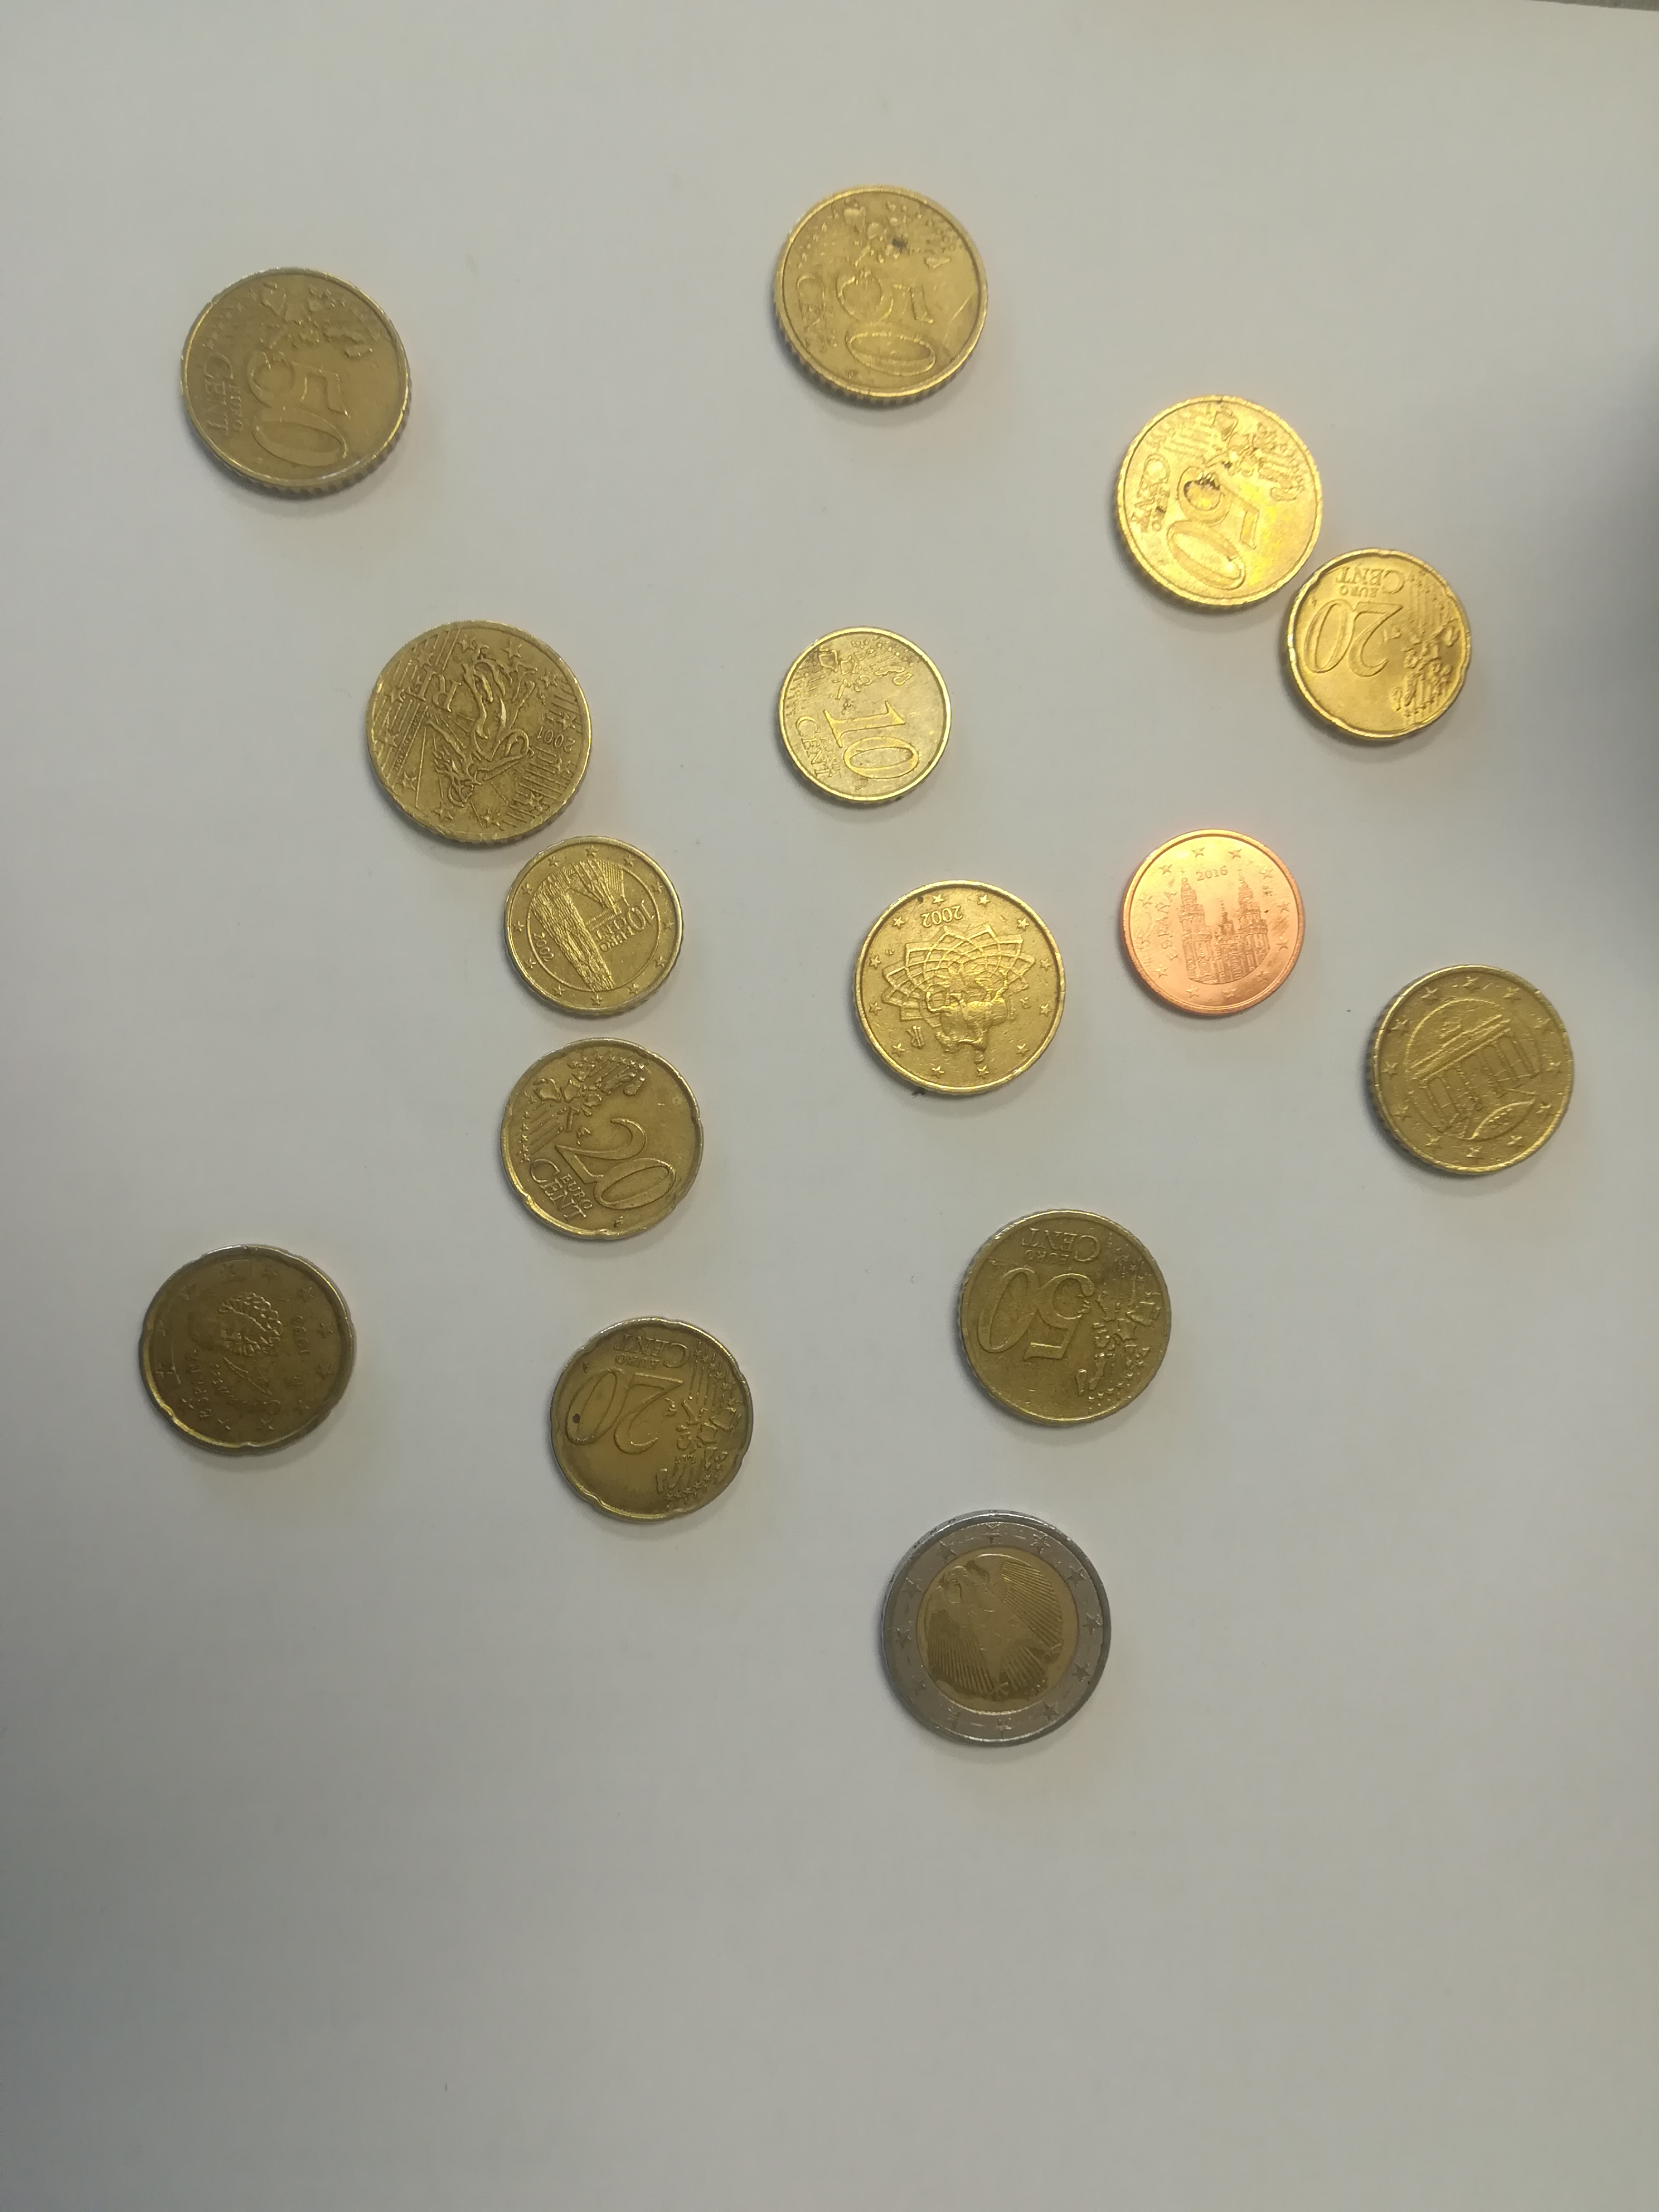
\includegraphics[width=0.4\linewidth]{images/15coins/manycoins.png}
\includegraphics[width=0.4\linewidth]{images/15coins/out_manycolors.png}
\end{center}

Remarquons que le fond de l'image est correctement détecté, et c'est tout ce qui importe. Nous allons maintenant voir comment exploiter cette information pour compter le nombre de pièces.

\subsection{Deuxième passe: pièces de monnaie}
\subparagraph{}
Une fois que nous avons réussi à détecter le fond, nous pouvons séparer le graphe en deux parties: le fond et les pièces. Ceci peut être fait avec un algorithme trivial que nous ne détaillerons pas ici. Voici le résultat que l'on obtient:

\begin{center}
\includegraphics[width=0.4\linewidth]{images/15coins/out_manycolors.png}
\includegraphics[width=0.4\linewidth]{images/15coins/out_2colors.png}
\end{center}

\subparagraph{}
Maintenant, il ne reste plus qu'à détecter les pièces individuelles. Pour ce faire, il suffit calculer les composantes connexes du sous-graphe contenant les pièces, toujours avec un DFS. Pour ce faire, nous connectons les pixels adjacents s'ils appartiennent au même sous-graphe. Nous ne détaillons pas le code mais une version commentée se trouve en annexe. Nous n'accordons alors plus aucune importance à la couleur, la distinction entre le fond et les pièces ayant déjà été faite par la première passe. Le résultat obtenu est alors le suivant. De nouveau, des couleurs générées aléatoirement ont été utilisées pour aider à la visualisation:

\begin{center}
\includegraphics[width=0.4\linewidth]{images/15coins/out_2colors.png}
\includegraphics[width=0.4\linewidth]{images/15coins/out_chunks.png}
\end{center}

\subparagraph{}
C'est bien le résultat attendu, il suffit maintenant de compter le nombre de composantes connexes détectées parmi les pièces. Sur cette image, la réponse est évidemment... $1202$ !? L'image a l'air correcte à priori, comment se fait-il que l'algorithme détecte $1202$ pièces et non $15$ ? Une analyse détaillée de l'image révèle de toutes petites taches de couleur et lorsqu'on demande au programme d'afficher la taille des différentes composantes connexes on se rend compte que certaines ont une taille de $20$ pixels ou moins.

\subsection{Filtrage heuristique}
\subparagraph{}
Afin de déterminer quelles composantes connexes correspondent ou non à des pièces de monnaie, nous allons appliquer deux heuristiques. Premièrement, nous pouvons éliminer les composantes connexes d'une taille en pixels inférieure à $t\%$ de l'image, avec $t$ que nous appellerons coefficient de tolérance. Une valeur de $t=0.1$ fonctionne assez bien. Cela peut sembler peu mais pour une image de $12000000$ pixels, cela veut dire que les pièces doivent faire au moins $1200$ pixels, ce qui n'est pas négligeable. Avec cette modification, notre algorithme détecte correctement les $15$ pièces de monnaie.

\subparagraph{}
Deuxièmement, nous pouvons éliminer les composantes connexes qui n'ont pas la forme d'une ellipse. Bien qu'il n'ait pas fallu recourir à cette option pour cette image-ci, cela se révèle souvent nécessaire en pratique. Nous avons par exemple essayé d'appliquer notre algorithme à l'image ci-dessous. Le résultat est assez clair:

\begin{center}
\includegraphics[width=0.4\linewidth]{images/4coins/img3.png}
\includegraphics[width=0.4\linewidth]{images/4coins/out_chunks.png}
\end{center}

Une approximation qui fonctionne assez bien en pratique est de calculer les valeurs minimale et maximale de $x$ et de $y$ pour tous les points appartenant à une composante connexe donnée. Nous pouvons alors calculer une approximation de l'aire sur base de ces valeurs en partant du principe que la forme repérée est une ellipse:
$$A = \frac{\pi}{4}\cdot |x_{min} - x_{max}|\cdot|y_{min} - y_{max}|$$.
Une fois cette aire calculée, nous pouvons comparer cette valeur à la taille en pixels de la composante connexe et nous assurer que l'erreur est bien inférieure à un certain pourcentage. Nous avons choisi $20\%$ mais une valeur plus faible aurait sans doute fait l'affaire.

\subsection{Complexité}
\subparagraph{}
La complexité d'un algorithme est définie comme la quantité de ressources (temps ou mémoire) nécessaire à son exécution. La notation $\mathcal O(\ldots)$ exprime la complexité asymptotique d'un algorithme dans le pire cas, où $\ldots$ est fonction d'un certain nombre de paramètres.

\subparagraph{}
Si nous prenons $w$ la largeur de l'image à analyser et $h$ sa hauteur, notre algorithme tourne en un temps $\mathcal O(wh)$. Posons $n = wh$ par simplicité. Chacun des DFS prend $\mathcal O(n + 4n) = \mathcal O(n)$. En effet, chaque sommet est visité une fois ($\mathcal O(n)$) et pour chaque sommet il faut tester les $4$ potentiels sommets adjacents ($\mathcal O(n)$). Les heuristiques sont aussi en $O(n)$ car elles nécessitent de parcourir tous les pixels exactement une fois. Notre algorithme tourne donc en $\mathcal O(n)$ et il est trivial de constater qu'il utilise $\mathcal O(n)$ en mémoire. Il est d'ailleurs impossible d'obtenir une complexité inférieure à partir du moment où on souhaite lire toute l'image, car la lecture prend au moins $\mathcal O(n)$ en temps et en mémoire. La partie la plus lente de notre programme est sans doute le chargement et la sauvegarde des images, car la bibliothèque utilisée pour ça doit suivre des algorithmes bien plus compliqués pour décoder et surtout encoder efficacement l'image. Pour garantir une complexité de $\mathcal O(n)$, nous pourrions utiliser un format de fichier non compressé comme les \textit{bitmaps} (.bmp) mais cela ne semble pas nécessaire en pratique et nous ne l'avons donc pas fait.